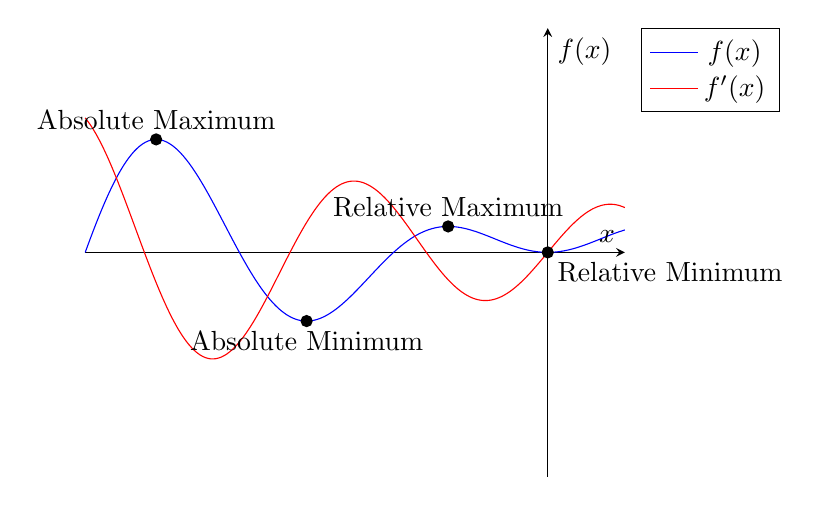
\begin{tikzpicture}
		\begin{axis}[
				axis lines        = center,
				xmin              = -3,
				xmax              = 0.5,
				ymin              = -5,
				ymax              = 5,
				xlabel            = $x$,
				xtick             = \empty,
				ylabel            = $f(x)$,
				ytick             = \empty,
				variable          = t,
				trig format plots = rad,
				legend pos        = outer north east,
				clip              = false
			]

			\addplot [
				domain  =-3:0.5,
				color   =blue,
				samples = 100,
				smooth,
			]
			{x * sin(pi * x)};
			\addlegendentry{$f(x)$}

			\addplot [
				domain  =-3:0.5,
				color   =red,
				samples = 100,
				smooth
			]
			{sin(pi * x) + x * cos(pi * x)};
			\addlegendentry{$f'(x)$}

			\addplot [
				only marks,
				color=black,
				mark=*
			]coordinates {(-2.54,2.52)(-1.564,-1.532)(-0.646,0.579)(0,0)};

			\node[above] at (-2.540, 2.520) {Absolute Maximum};
			\node[below] at (-1.564, -1.532) {Absolute Minimum};
			\node[above] at (-0.646, 0.579) {Relative Maximum};
			\node[below right] at (0, 0) {Relative Minimum};
		\end{axis}
	\end{tikzpicture}
